\clearpage

\lehead[]{\sf\hspace*{-2.00cm}\textcolor{white}{\colorbox{lightblue}{\parbox[c][0.70cm][b]{1.60cm}{
\makebox[1.60cm][r]{\thechapter}\\ \makebox[1.60cm][r]{ÜBUNG}}}}\hspace{0.17cm}\textcolor{lightblue}{\chaptertitle}}
\rohead[]{\textcolor{lightblue}{\chaptertitle}\sf\hspace*{0.17cm}\textcolor{white}{\colorbox{lightblue}{\parbox[c][0.70cm][b]{1.60cm}{\thechapter\\
ÜBUNG}}}\hspace{-2.00cm}}
%\chead[]{}
\rehead[]{\textcolor{lightblue}{AvHG, Inf, My}}
\lohead[]{\textcolor{lightblue}{AvHG, Inf, My}}

\section{Programmierübung zur Haustierdatenbank}

\subsection{Aufgabe 1: Ausgabe mit einer JList-Komponente}

Zeige in einer \myClass{JList}-Komponente alle Besitzer mit ihren Tieren an,
sofern die Tiere noch lebendig sind. Die Ausgabe soll nach dem folgenden Schema erfolgen:

\myUserInput{Besitzer-Nachname, Besitzer-Vorname: Tiername, Tierart, Tier-Geschlecht}

Sortiere die Ausgabe nach dem Nachnamen des Besitzers.

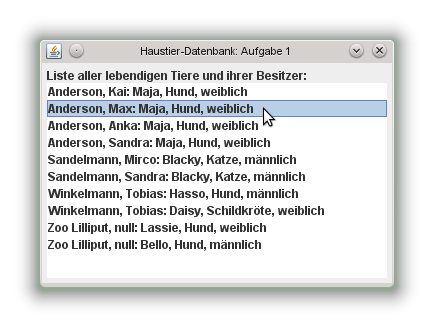
\includegraphics[width=0.5\textwidth]{./inf/SEKII/37_JavaSQL_Datenbankzugriffe/HaustierAufgabe1.png}


\subsection{Aufgabe 2: Datensätze durchblättern}

Im Fenster werden jeweils die Daten eines Tieres angezeigt. Zu Beginn werden die
Daten des Tieres mit der Tiernummer 1 geladen.
Über einen „Vorwärts“-Button gelangt der Benutzer zu den Daten des Tieres mit
der nachfolgenden Tiernummer. Über einen „Rückwärts“-Button gelangt der Benutzer
zu den Daten des Tieres mit der vorhergehenden Nummer. Wenn es zu einer id
keinen Datensatz gibt, dann soll die id mit anderweitig leeren Textfeldern
angezeigt werden.

\begin{minipage}{0.3\textwidth}
Die Button Vorwärts und Zurück werden deaktiviert, wenn es keinen vorherigen
bzw. nachfolgenden Datensatz gibt. Dazu muss zu Beginn des Programms die Anzahl
der vorhandenen Tiere abgefragt werden.
\end{minipage}
\begin{minipage}{0.7\textwidth}
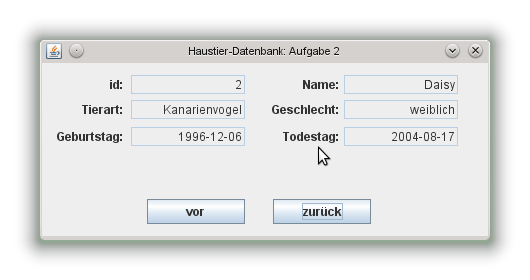
\includegraphics[width=1.0\textwidth]{./inf/SEKII/37_JavaSQL_Datenbankzugriffe/HaustierAufgabe2.png}
\end{minipage}

Alle Textfelder sollen nicht-editierbar sein.

\subsection{Aufgabe 3: Tiere löschen}

\begin{minipage}{0.5\textwidth}
Der Benutzer kann die Tiernummer eines Tieres eingeben, das gelöscht werden
soll. Wenn der Benutzer den „Löschen“-Button drückt, erscheint zunächst eine
Sicherheitsabfrage (z.B: „Wollen Sie das Tier mit der Nummer 2 wirklich
löschen?“). Nach einer positiven Bestätigung werden der Tiereintrag und alle
Verweise auf das Tier in der Beziehungstabelle gelöscht.
\end{minipage}
\begin{minipage}{0.5\textwidth}
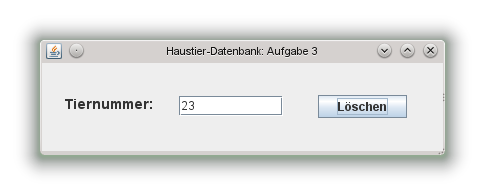
\includegraphics[width=1.0\textwidth]{./inf/SEKII/37_JavaSQL_Datenbankzugriffe/HaustierAufgabe3.png}
\end{minipage}

Achtung: Man kann ein Tier nicht löschen, wenn es in der Beziehungstabelle
referenziert ist (durch das Löschen würde in der Beziehungstabelle ansonsten
ein Toter Verweis entstehen. Man sagt: \emph{Die referenzielle Integrität würde
verletzt.})

Es gibt nun zwei Möglichkeiten: entweder müssen zunächst alle Einträge in der
Tabelle \myUserInput{beziehung}, die sich auf das zu löschende Tier beziehen
entfernt (gelöscht) werden, oder man erweitert die Definition des
Fremdschlüssels wie folgt:

\begin{lstlisting}
FOREIGN KEY (beziehung_tier_id) REFERENCES tier (tier_id) ON DELETE CASCADE
\end{lstlisting}

Durch den Zusatz \lstinline|ON DELETE CASCADE| wird MySQL angewiesen auch die
betroffenen Einträge in der Beziehungstabelle zu löschen, wenn ein Tier
gelöscht wird. Dieser Automatismus ist zum einen bequem, zum anderen aber auch
höchst gefährlich, weshalb die Verwendung dieser Technik in vielen Unternehmen
auch verboten ist.
\subsection{Aufgabe 4: Neue Tiere hinzufügen}

Im Fenster können die Daten eines neuen Tieres angelegt werden. Es gibt
Eingabefelder für jeden Datumswert und einen „Hinzufügen“-Button. Wenn der
Benutzer auf den Button drückt, wird ein neues Tier mit den von ihm eingegebenen
Daten angelegt. Falls der Benutzer keinen Todestag angegeben hat, soll für den
Todestag der Wert \myUserInput{NULL} eingefügt werden.

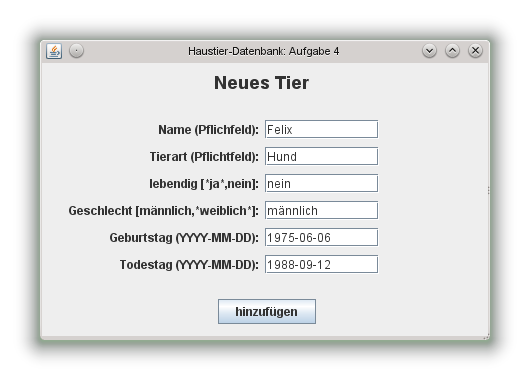
\includegraphics[width=0.5\textwidth]{./inf/SEKII/37_JavaSQL_Datenbankzugriffe/HaustierAufgabe4.png}


